\documentclass{article}

\usepackage[english]{babel}

% Set page size and margins
% Replace `letterpaper' with `a4paper' for UK/EU standard size
\usepackage[a4paper,top=2cm,bottom=2cm,left=3cm,right=3cm,marginparwidth=1.75cm]{geometry}

% Useful packages
\usepackage{amssymb}
\usepackage{siunitx}
\PassOptionsToPackage{hyphens}{url}\usepackage{hyperref}
\usepackage{cleveref}
\usepackage{float}
\usepackage[utf8]{inputenc}
\usepackage[right]{lineno}
\usepackage{csquotes}
\usepackage{booktabs}
\usepackage{longtable}
\usepackage{adjustbox}
\usepackage{array}
\usepackage{url}
\usepackage{titlesec}
%\usepackage[compatibility=false]{caption}
\usepackage{authblk}
\usepackage{xcolor} % Load the xcolor package for color options
\renewcommand{\thetable}{\Roman{table}}

% Define a new format for \subsection
\titleformat{\subsection}
  {\mdseries\itshape\large} % Medium series, italic shape, and large font size
  {\thesubsection}{1em}{} % Numbering, spacing, and the section title itself


% Emerald Harvard Citation Style

\usepackage[english]{babel}
\usepackage[style=authoryear,backend=biber,natbib=true,maxcitenames=2,uniquelist=false]{biblatex}
\addbibresource{Bibliography.bib} % your .bib file

% Customizing biblatex for Harvard style
% Customizing biblatex for Harvard style
\DeclareNameAlias{sortname}{family-given}
\DeclareNameAlias{default}{family-given}

\renewbibmacro{in:}{}
\DeclareFieldFormat[article]{title}{\mkbibquote{#1}\addcomma}
\DeclareFieldFormat[book]{title}{\mkbibemph{#1}\addcomma}
\DeclareFieldFormat[bookinbook]{title}{\mkbibemph{#1}\addcomma}
\DeclareFieldFormat[inbook]{title}{\mkbibquote{#1}\addcomma}
\DeclareFieldFormat[incollection]{title}{\mkbibquote{#1}\addcomma}
\DeclareFieldFormat[inproceedings]{title}{\mkbibquote{#1}\addcomma}
\DeclareFieldFormat[manual]{title}{\mkbibemph{#1}\addcomma}
\DeclareFieldFormat[misc]{title}{\mkbibemph{#1}\addcomma}
\DeclareFieldFormat[thesis]{title}{\mkbibemph{#1}\addcomma}
\DeclareFieldFormat[unpublished]{title}{\mkbibquote{#1}\addcomma}
\DeclareFieldFormat[patent]{title}{\mkbibemph{#1}\addcomma}
\DeclareFieldFormat[report]{title}{\mkbibemph{#1}\addcomma}
\DeclareFieldFormat[online]{title}{\mkbibquote{#1}\addcomma}
\DeclareFieldFormat[software]{title}{\mkbibemph{#1}\addcomma}
\DeclareFieldFormat[booklet]{title}{\mkbibemph{#1}\addcomma}
\DeclareFieldFormat[periodical]{title}{\mkbibemph{#1}\addcomma}
\DeclareFieldFormat[standard]{title}{\mkbibemph{#1}\addcomma}

\DeclareFieldFormat[article]{journaltitle}{\iffieldundef{shortjournal}{\mkbibemph{#1}\addcomma}{\mkbibemph{\printfield{shortjournal}}\addcomma}}
\DeclareFieldFormat{volume}{\bibstring{volume}~#1}
\DeclareFieldFormat{number}{\bibstring{number}~#1}

% Definitions for "Vol." and "No."
\DefineBibliographyStrings{english}{
  volume = {Vol.},
  number = {No.}
}

\renewbibmacro*{volume+number+eid}{%
  \printfield{volume}%
  \setunit*{\addspace}%
  \printfield{number}%
  \setunit{\addcomma\space}%
  \printfield{eid}}

\renewbibmacro*{journal+issuetitle}{%
  \usebibmacro{journal}%
  \setunit*{\addcomma\space}%
  \usebibmacro{volume+number+eid}%
  \setunit{\addcomma\space}%
  \usebibmacro{issue+date}}

\renewbibmacro*{publisher+location+date}{%
  \printlist{publisher}%
  \iflistundef{location}
    {\setunit*{\addcomma\space}}
    {\setunit*{\addcolon\space}}%
  \printlist{location}%
  \setunit*{\addcomma\space}%
  \usebibmacro{date}}

\renewcommand*{\bibpagespunct}{\addcomma\space}

% Customizing page field format to prevent duplication
% \DeclareFieldFormat{pages}{%
%   \mkfirstpage[{\mkpageprefix[page]{#1}}]{#1}}

% Customizing citations for Harvard style
\DeclareCiteCommand{\cite}[\mkbibparens]
  {\usebibmacro{prenote}}
  {\usebibmacro{citeindex}%
   \usebibmacro{cite}}
  {\multicitedelim}
  {\usebibmacro{postnote}}

\renewbibmacro*{cite:labelyear+extrayear}{%
  \iffieldundef{labelyear}
    {}
    {\printtext[bibhyperref]{%
       \printfield{labelyear}%
       \printfield{extrayear}}}}

\renewbibmacro*{cite:labeldate+extradate}{%
  \iffieldundef{labelyear}
    {}
    {\printtext[bibhyperref]{%
       \printfield{labelyear}%
       \printfield{extradate}}}}

\AtEveryBibitem{
  \clearfield{month}
  \clearfield{day}
  \ifentrytype{book}{
    \clearlist{location}
  }{}
}

% Formatting "et al." in italics followed by a comma
\DefineBibliographyStrings{english}{
  andothers = {\textit{et al.},}
}

\DeclareFieldFormat[article]{volume}{\bibstring{jourvol}\addnbspace #1}
\DeclareFieldFormat[article]{number}{\bibstring{number}\addnbspace #1}
\DeclareFieldFormat[article]{volume}{Vol. #1}
\DeclareFieldFormat[article]{number}{No. #1}
% Customizing DOI field format to lowercase "doi"
%\DeclareFieldFormat{doi}{\bibstring{doi}\addcolon\space\url{#1}}

% Customizing URL field format to "available at:"
\DeclareFieldFormat{url}{\bibstring{available at}\addcolon\space\url{#1}}
\DeclareFieldFormat{urldate}{\mkbibparens{accessed \addspace#1}}

% Customizing urldate to match the required format
\DeclareFieldFormat{urldate}{%
  \mkbibparens{accessed\space%
    \thefield{urlday}\addspace%
    \mkbibmonth{\thefield{urlmonth}}\addspace%
    \thefield{urlyear}}}


% Configure cleveref
\crefformat{figure}{#2Figure~#1#3}
\Crefformat{figure}{#2Figure~#1#3}
\crefformat{table}{#2Table~#1#3}
\Crefformat{table}{#2Table~#1#3}
\crefformat{section}{#2Section~#1#3}
\Crefformat{section}{#2Section~#1#3}

%Front Matter
\author[1]{Arceta, Althea Zyrie}
\author[2]{Tan, Jose Tristan}
\author[3]{Tumalad, Shawne Michael}

\affil[1]{althea\_arceta@dlsu.edu.ph}
\affil[2]{tristan\_tan@dlsu.edu.ph}
\affil[3]{shawne\_tumalad@dlsu.edu.ph}

\title{Exercise 1: Keyword Spotting}

\begin{document}

\maketitle

\section{Introduction}
\label{sec:introduction}
Keyword spotting (KWS) is a useful technique for speech applications that allows users to activate devices by simply saying a keyword phrase. Recent advancements in deep learning have significantly improved the accuracy and efficiency of KWS models, making them suitable for integration into even small electronic devices and web browsers.

This exercise aims to explore the design, training, and deployment of a keyword-spotting neural network using TinyML hardware and Edge Impulse. The primary objective is to build a simple neural network model capable of recognizing specific keywords or phrases and deploying it on TinyML. This exercise serves to familiarize us with the fundamentals of TinyML, including dataset creation, model design, and on-device inference.

\section{Background and Related Work}
\label{sec:bg_and_rw}
New technology keeps emerging every day. Slowly integrating and changing how we live, work, and communicate, making our lives significantly easier. However, as we grew more and more accustomed to technology, we became more and more dependent on technology. Hence, the demand for communication between humans and computers has never been greater. Speech recognition is one example of this technology, which allows computers to understand and analyze verbal messages. This technology is applied to applications across various domains, from virtual assistants to automated transcription services. However, while speech recognition offers high potential, its implementation often demands high computational resources and memory. This can be challenging for edge devices with limited capabilities \cite{SpeechRecog}. Based on the following scenario, keyword spotting (KWS) can aid in addressing the resource limitations at the edge devices.

Keyword spotting (KWS) is a technique for speech applications that allows users to activate devices by simply saying a keyword phrase \cite{10528680}. Examples of wake-up words include 'Alexa,'\cite{Amazon} 'Hey Siri,'\cite{Siri} and 'Okay, Google' \cite{Google}. Additionally, advancements in artificial intelligence (AI) have significantly improved human-machine interaction, especially with technologies that convert speech into executable actions \cite{KHEDDAR2024102422}.

However, as the demand for smarter, more responsive devices grows, more and more technologies are being developed to meet this demand. We have now reached a stage where AI applications can be deployed on compact, low-power devices without external servers. This marks the foundation of Tiny Machine Learning (TinyML), a breakthrough that enables efficient, real-time AI processing directly on edge devices.

TinyML, unlike conventional fashions that depend on powerful cloud-based virtual servers for processing, brings intelligence at once to facet gadgets, which include microcontrollers and Internet of Things (IoT) devices. This decentralized technique enables actual-time choice-making without consistent reliance on external servers \cite{TNML}. TinyML works by quantizing the AI model to reduce its overall size so that it can be deployed on edge devices. This, of course, decreases accuracy, so it is part of development to optimize the model for the given microcontroller's constraints and computational power. TinyML devices can be configured to adapt and enhance themselves as time passes, ensuring the model stays updated and powerful.

TinyML is scalable, energy efficient, private, and performs in real-time. As the devices used for TinyML are small and typically excluded from the cloud, such advantages are effective in many technological sectors. A well-known example would be smartwatches, which implement TinyML in their programs for tasks such as health monitoring. Similarly, the Arduino Nano 33 BLE, which is used in this exercise, brings these benefits to an accessible platform, allowing TinyML applications to run efficiently on small devices. Its low power consumption and real-time processing capabilities make it suitable for various applications, such as edge AI applications.

The edge AI platform used in this exercise is Edge Impulse. Edge Impulse is a suite of tools that helps you build, test, and deploy edge AI algorithms. It covers the entire workflow, from data collection to model optimization and production monitoring. Edge Impulse increases the velocity of edge AI development while reducing costs and associated risks \cite{EDGE}. It simplifies the process of bringing AI and machine learning to edge devices, allowing developers to create intelligent applications that can run on small, energy-efficient hardware. 

TinyML is poised to revolutionize the way AI operates at the edge, enabling smarter, more responsive devices that can function independently of cloud servers. With its scalable, energy-efficient, and privacy-focused approach, TinyML brings intelligence to microcontrollers and IoT devices, empowering real-time decision-making in a variety of applications. As this technology continues to evolve, it will undoubtedly become a cornerstone of future innovations, shaping the landscape of AI-driven solutions for years to come.

\section{Methodology}
\label{sec:methodology}
When creating a keyword spotting system, start by selecting a keyword to recognize. Consider how multi-syllable words (like "Hello world") outperform single-syllable words. For our group, the selected keywords are 'Talk to me,' 'Wake up,' and 'Hey Duino.'

\begin{enumerate}
  \item Setting up: open the platform's website and log in to your account. If you haven't already done so, create a new account. Once logged in, navigate to the project creation page and establish a new project.
  \item Data Collection: Record 10s to 60s audio samples using the selected keywords, ensuring pauses between every keyword. After, use the 'Split Sample' to split the audio into segments. Repeat the process till there are at least 10 minutes of samples per class. Additionally, it is crucial to ensure that the samples include a variety of speakers with different genders, ages, accents, and vocal characteristics. This diversity will help the model generalize better across different user profiles and improve overall performance in real-world conditions.
  \item Noise and Unknown: In addition to your keyword, we'll also need audio that is not your keyword. Like background noise, the TV playing ('noise' class), and humans saying other words ('unknown' class). Add pre-built datasets for 'noise' and 'unknown' classes to our dataset.
  \item Balancing the Dataset: Select Perform train/test split by going to Dashboard. This will automatically split your data between a training class (80\%) and a testing class (20\%).
    \begin{figure}[H]
        \centering
        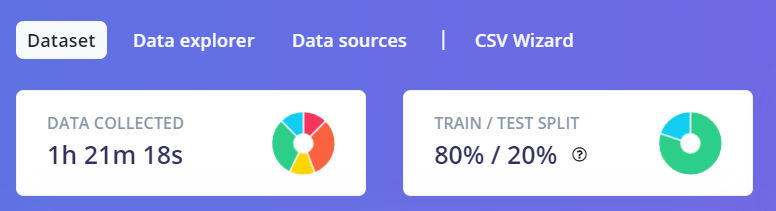
\includegraphics[width=8cm]{Figures/balance_ds.png}
        \caption{Balanced Dataset}
        \label{fig:balancedt}
    \end{figure}
  \item Impulse Design: In the Create impulse tab, add Time series data, an Audio (MFCC), and a Classification (Keras) block. Leave the window size to the length of the keyword audio samples (in our case, 1000ms or 1 second) and click Save Impulse.
    \begin{figure}[H]
        \centering
        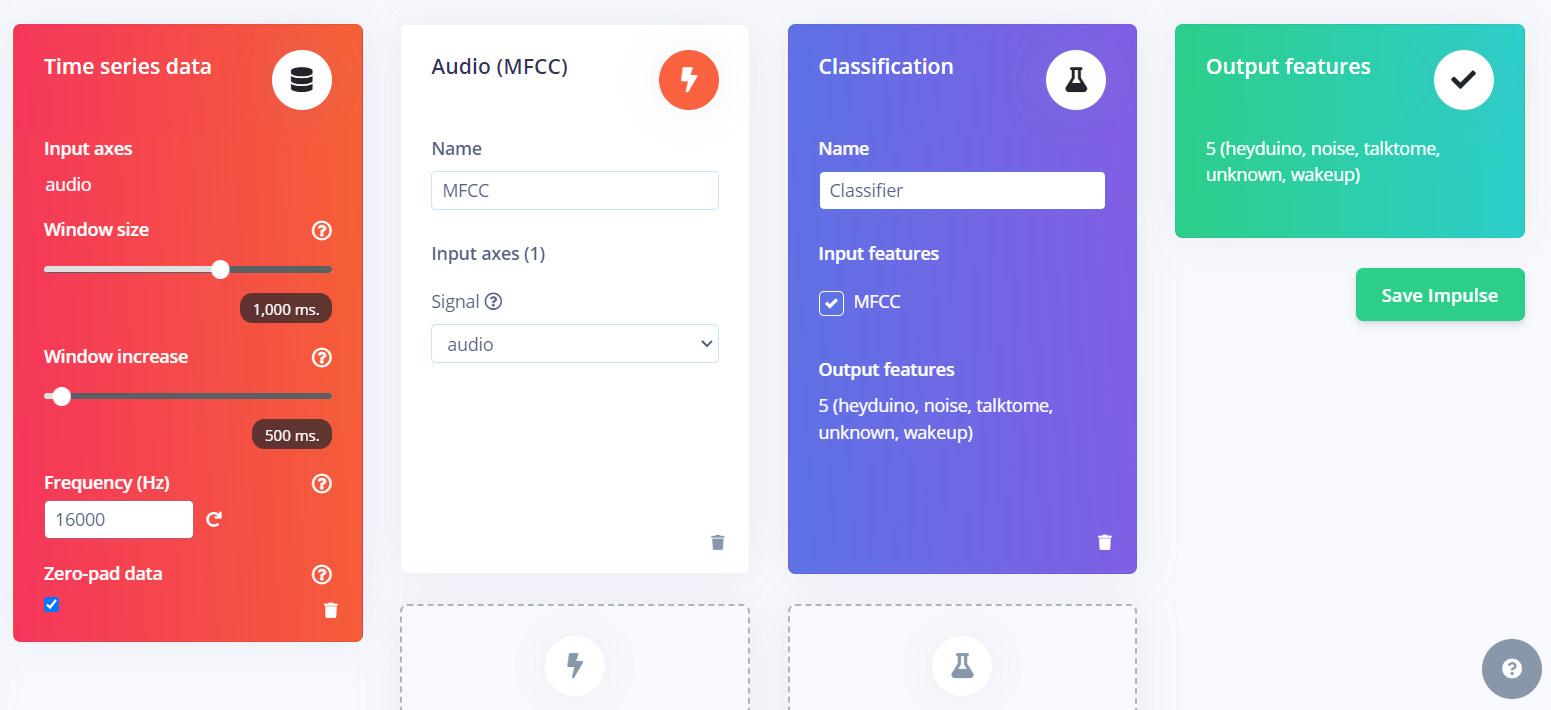
\includegraphics[width=8cm]{Figures/impulseDesign.png}
        \caption{Impulse Design Parameters}
        \label{fig:impulse}
    \end{figure}
  \item Configuration of the MFCC block: After assembling the building blocks of our Impulse, click on the MFCC tab in the navigation menu on the left-hand side. In our case, we stuck to the default parameters.
    \begin{figure}[H]
        \centering
        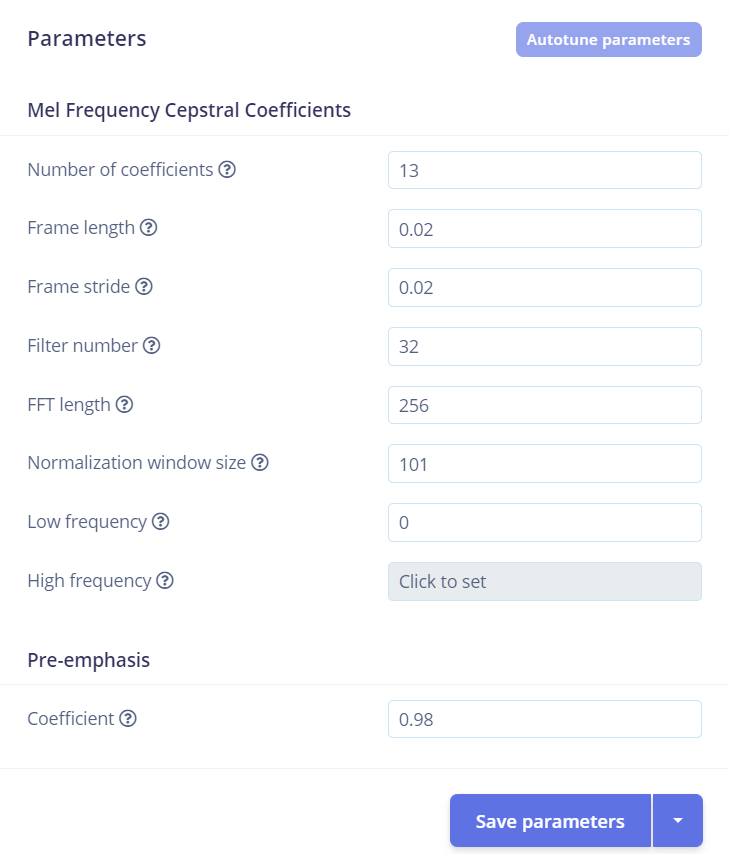
\includegraphics[width=8cm]{Figures/mfcc_config.png}
        \caption{MFCC Block Configuration}
        \label{fig:mfcc}
    \end{figure}
    
  \item Neural Network: With all data processed, it's time to start training a neural network. The network that we're training here will take the MFCC as an input. Configure the settings based on your choice on the NN Classifier tab. 
    \begin{figure}[H]
        \centering
        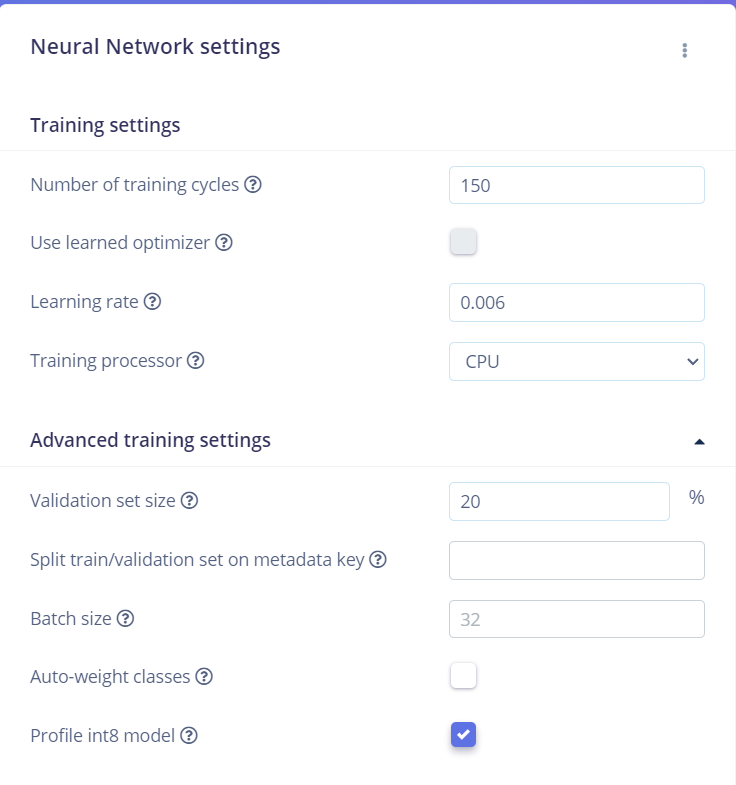
\includegraphics[width=8cm]{Figures/nna(1).png}
        \caption{Neural Network Settings (1)}
        \label{fig:nna1}
    \end{figure}

    \begin{figure}[H]
        \centering
        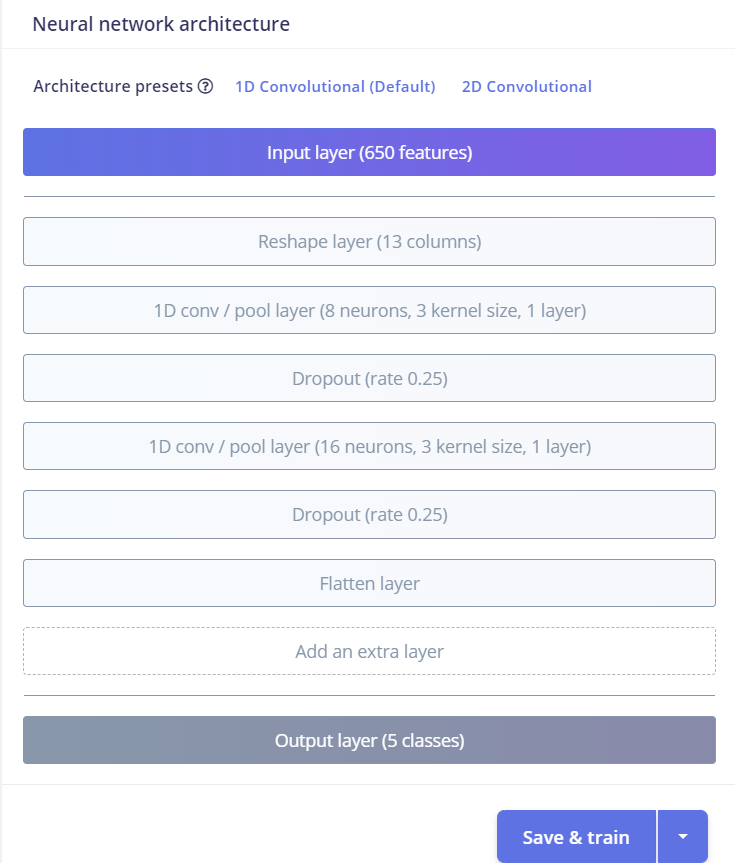
\includegraphics[width=8cm]{Figures/nna(2).png}
        \caption{Neural Network Settings (2)}
        \label{fig:nna2}
    \end{figure}
  \item Testing and Validation: With everything in place, click Start training. Training will take a few minutes. When it's complete, the Last training performance panel appears at the bottom of the page. After, make sure to inspect and correct any misclassified samples or labels.

    \begin{figure}[H]
        \centering
        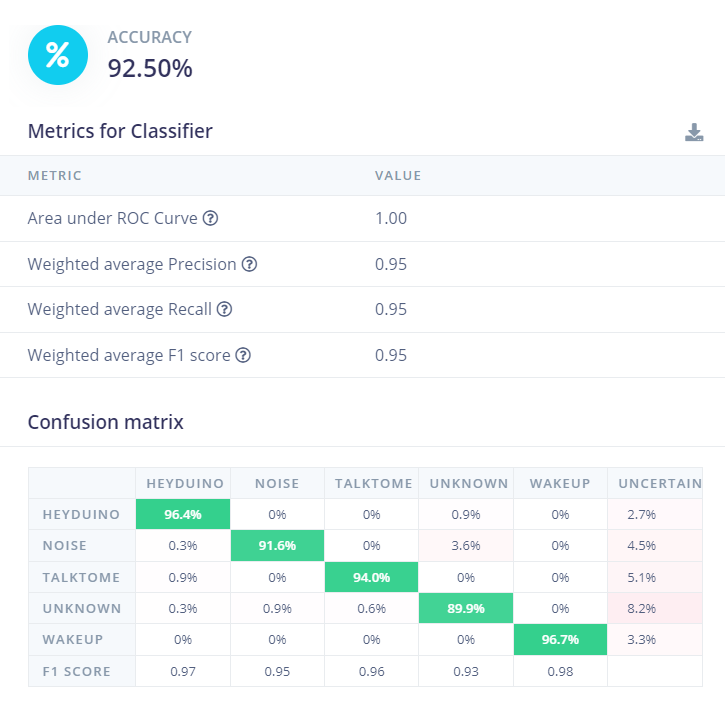
\includegraphics[width=8cm]{Figures/test_acc.png}
        \caption{Accuracy Result of the Test Dataset}
        \label{fig:testacc}
    \end{figure}

    \begin{figure}[H]
        \centering
        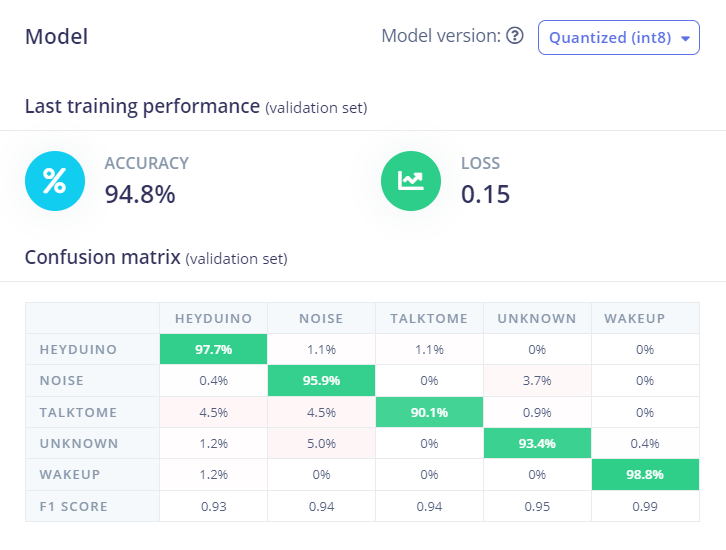
\includegraphics[width=8cm]{Figures/train_acc.png}
        \caption{Accuracy Result of the Train Dataset}
        \label{fig:trainacc}
    \end{figure}
  \item Deployment: After training the model, the model can be deployed to our TinyML Arduino Kit. In the Deployment tab, select 'Arduino Library' for Selected Development and configure the settings to your preferences. Click build to create a library that contains example code that can be deployed on an Arduino development board. 
  \item Verification: After deploying the sample code ('') on the development board, the system is tested through console output to verify that the system works. 
  \item LED: After verifying the system, the sample code (shown below) is augmented to modify the board's LED output based on the model's readings. 
  
  \begin{figure}[H]
        \centering
        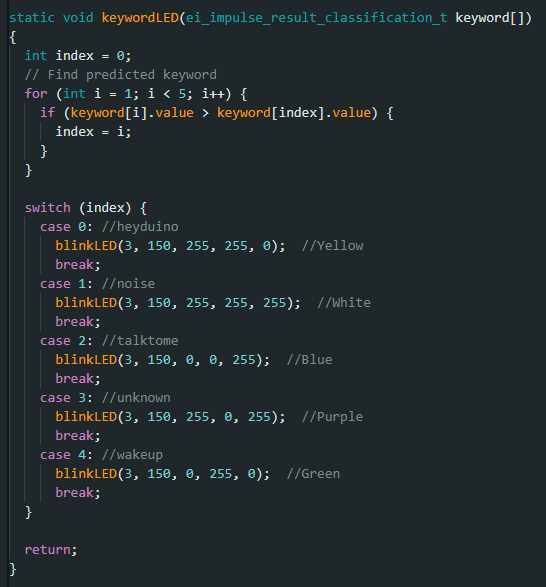
\includegraphics[width=8cm]{Figures/keywordLED.png}
        \caption{Code Snippet of keywordLED Function}
        \label{fig:ledKey}
  \end{figure}
  This is done by assigning an LED color to each keyword and blinking the LED color three times to correspond to the maximum keyword value. Below is the list of keywords and their respective LED colors.
  \begin{itemize}
      \item 'Hey Duino' - Yellow
      \item 'Talk to me' - Blue
      \item 'Wake up' - Green
      \item 'Noise' - White
      \item 'Unknown' - Purple
  \end{itemize}
    
\end{enumerate}

\section{Evaluation}
\label{sec:evaluation}

The model will be assessed based on accuracy, precision, recall, and on-device performance. We conducted tests under various circumstances to determine performance. The following metrics were gathered:

\begin{itemize}
    \item Accuracy: The percentage of correct predictions made by the model.  To evaluate the model's accuracy, the researchers will test the model with a dataset that includes training and unseen test data.
    \item Precision: How well the model distinguishes between similar-sounding words. To assess the model's precision, researchers will present the model with a series of phonetically similar words or phrases (e.g., "Hey Duino" vs. "Arduino") to determine if it correctly identifies the target keyword without mistakenly triggering similar sounds.
    \item Adaptability: The model's ability to generalize across different voice recordings. To assess the model's adaptability, researchers will test the model under varied test conditions, including voices with different pitch ranges, genders, and ages and recordings made in different environments (e.g., quiet rooms vs. noisy streets).
\end{itemize}

\section{Conclusion}
\label{sec:conclusion}

Overall, this exercise provided valuable hands-on experience designing, training, and deploying a TinyML keyword-spotting neural network using Edge Impulse. We successfully implemented a foundational model incorporating a personalized dataset, achieving accurate keyword recognition on a mobile device.

Future work could delve deeper into model optimization. We may obtain even higher accuracy by adding more data or fine-tuning the neural net architecture. These enhancements would make our keyword-spotting approach more accurate in real-world circumstances.

\printbibliography

\end{document}
